\documentclass[doc]{apa6} % APA style header

	\usepackage{apacite} % citations in APA style
	\usepackage[utf8]{inputenc} % force LaTeX to admit that ASCII is really not that great


% ---------- watermark -----------
\usepackage[firstpage]{draftwatermark}
\SetWatermarkAngle{0}
\SetWatermarkFontSize{0.25cm}
\SetWatermarkVerCenter{1.15cm}
\SetWatermarkLightness{0.5}
\SetWatermarkHorCenter{14cm}
\SetWatermarkText{\shortstack[l]{
Martire, K. A., Growns, B. and Navarro, D. J. (2018). What do the experts \\
know? Calibration, precision, and the wisdom of crowds among forensic \\
handwriting experts. Psychonomic Bulletin and Review, 25, 2346–2355 \\
https://doi.org/10.3758/s13423-018-1448-3
}}
\SetWatermarkScale{1}
% -------------------------------



	% title
	\title{What do the experts know? Calibration, precision, and the wisdom of crowds among forensic handwriting experts}

	% authors
	\threeauthors{\normalsize Kristy A. Martire}{\normalsize Bethany Growns}{\normalsize Danielle J. Navarro}
	\threeaffiliations{School of Psychology \\ University of New South Wales}{School of Psychology \\ University of New South Wales}{School of Psychology \\ University of New South Wales}

	% author note
	\authornote{Correspondence concerning this article should be sent to A/Prof. Kristy Martire. School of Psychology, The University of New South Wales, Sydney, NSW, 2052 Australia. This work was supported by ARC DECRA Fellowship to KAM (DE140100183). Thanks to Thomas Vastrick for providing database access and thoughtful comments on an earlier draft, Jonathan Berengut for his assistance with data representation, and Brigid Betz-Stablein from Stats Central. The authors declare that they had no conflicts of interest with respect to their authorship or the publication of this article. KAM developed the study concept and obtained access to the experimental stimuli.  The study was designed by KAM and BG, and programming was completed by BG. Analyses were performed by DJN, and all authors contributed to writing the manuscript.}

	% header
	\shorttitle{Calibration, precision and forensic expertise}

	% abstract
	\abstract{Forensic handwriting examiners currently testify to the origin of questioned handwriting for legal purposes. However, forensic scientists are increasingly being encouraged to assign probabilities to their observations in the form of a likelihood ratio. This study is the first to examine whether handwriting experts are able to estimate the frequency of US handwriting features more accurately than novices. The results indicate that the absolute error for experts was lower than novices, but the size of the effect is modest, and the overall error rate even for experts is large enough as to raise questions about whether their estimates can be sufficiently trustworthy for presentation in courts. When errors are separated into effects caused by miscalibration and those caused by imprecision, we find systematic differences between individuals. Finally, we consider several ways of aggregating predictions from multiple experts, suggesting that quite substantial improvements in expert predictions are possible when a suitable aggregation method is used.}


\begin{document}
	\maketitle
	\noindent
%\newpage

% ----------------------------------
\section{Introduction}

What makes someone an expert? On the one hand, legal scholarship and rules of evidence often cite the importance of knowledge, skill, experience, training, or education in a particular discipline (for example in Rule 702 of the {\it U.S. Federal Rules of Evidence}, 2016 and Section 79 of the Australian {\it Evidence Act (Cth)}, 1995; see \citeNP{Martire2017mar}). From a scientific perspective, both popular accounts \cite{gladwell2008outliers,ericsson2016peak} and scholarly literature on the development of expertise place an emphasis on the critical role of deliberate practice \cite{ericsson1993role}. Nevertheless, genuine expertise is more than mere experience: it should also produce expert {\it performance}, characterized as ``consistently superior performance on a specified set of representative tasks for a domain'' \cite[p. 277]{ericsson1996expert}. Yet in many situations ``performance'' is not at all straightforward to define, as there are very often no agreed upon ground truths or gold standards that can be used as the basis for assessment \cite{weiss2006people}. Indeed, this is the situation for many forensic science disciplines \cite{taroni2001finetti}.

An alternative approach suggests that expertise can be characterized in terms of the ability to make fine-grained discriminations in a consistent manner, as captured by measures such as the Cochran-Weiss-Shanteau (CWS) index \cite{weiss2003empirical}. This approach is appealing insofar as it can be applied even when objective gold standards are not available, but has one substantial drawback: it characterizes expertise in terms of the {\it precision} (i.e., discriminability and consistency) of expert performance rather than the {\it accuracy} (i.e., correctness).

One might hope that precision and accuracy are related, but in real life there are no guarantees that this is so. Whether one is considering the widespread belief in phrenology in the 19th century \cite{faigman2007anecdotal}, disproportionate trust in unreliable  \cite{saks2005coming} or unvalidated forensic methods \cite{PCAST2016}, beliefs in conspiracy theories \cite{goertzel1994belief} or ``groupthink'' that plagues decision making processes \cite{janis1982groupthink}, it is clear that communities of people can come to considerable agreement about incorrect claims. A phrenologist might indeed produce very precise judgments, making fine-grained discriminations about a person's character in a consistent way based on their physiognomy, but that does not mean the judgments of phrenologists are sufficiently accurate to be considered {\it expert} in a scientific sense. From a practical standpoint, therefore, the distinction between the precision of an individual and the accuracy of their judgments is of critical importance.

In this paper we explore this question in a real world domain, using forensic handwriting expertise as our testing ground. The domain is one of considerable practical importance: forensic handwriting examinations can be used to establish the origin of a questioned sample of handwriting for legal purposes \cite{dyer2006visual}, and these judgments can be accorded considerable weight at trial. The task is heavily reliant on subjective judgment, with human examiners completing these assessments via visual comparison of handwriting samples \cite{dror2010forensicexpertise}. Traditionally handwriting and other feature-comparison examiners (e.g., fingerprint) have been permitted to make categorical judgments (`match' or `no-match') without providing information about the uncertainty associated with their conclusion. Past research has suggested that forensic handwriting examiners are remarkably accurate in their ability to make these types of authorship determinations \cite<e.g.,>{sita2002forensic,found2008probative,kam2001signature}.

However, in the United States, the President's Council of Advisors on Science and Technology \citeyear{PCAST2016} and the National Academies of Science \citeyear{Edwards2009} have both strongly criticized the traditional approach -  arguing that unqualified categorical opinions are scientifically unsupportable. Consistent with these criticisms, many forensic scientists now endorse the use of likelihood ratios - the relative probability of the observations under different hypotheses as to their provenance - as the appropriate method for providing expert testimony \cite{Aitkin2011}. As part of adopting this approach, handwriting examiners may be called upon to observe handwriting features and then assign probabilities to feature occurrence if, for example, two handwriting samples originated from the same versus different writers \cite{dror2016hierarchy}. How plausible is it that human handwriting experts are capable of producing genuinely superior performance than novices on this task?

On the one hand, there is cause for optimism: research examining visual statistical learning reveals that people can automatically and unconsciously learn statistical relationships from visual arrays given relatively limited exposure \cite{Fiser2001,fiser2002,turkbrowne2005}. Further, experts have previously been found to have enhanced domain-specific statistical learning in comparison to novices \cite{schon2011musicalexpertise}. Indeed, it has sometimes been argued that the relevant probabilities (e.g., of seeing a particular handwriting feature given that two writing samples originated from the same versus different writers) can be estimated by the examiner based on their subjective experiences \cite{Biedermann2013}. On the other hand, the applied problem is essentially a probability judgment task, and there is considerable evidence that people tend not to be well calibrated at such tasks (e.g., \citeNP{lichtenstein1982calibration}, but see \citeNP{murphy1984impacts} in contexts where feedback is fast and accurate). Accordingly, there is some uncertainty as to whether forensic examiners will possess the relevant expertise in a fashion that would justify the use of such judgments in a legal context.

Our goal in this paper is to present the first empirical data examining this question, and in doing so, highlight the importance of distinguishing precision from accuracy in the assessment of expert performance. Our approach relies on a recently collected database of handwriting features \cite{johnson2016measuring}. This database was funded by the US National Institute of Justice (NIJ) to statistically estimate the frequency of handwriting features in a sample representative of the US adult population. We were able to access the estimates before they became publicly available. This allowed us to rely on a measure of ``ground truth'' that was not yet available to experts in the field. Using this database we were able to compare the performance of experts and novices, as well as people with high exposure to the relevant stimulus domain (US participants) and those whose experience pertains to a potentially different set of environmental probabilities (non-US participants).


% insert the accuracy figure
\begin{figure}[p]
\begin{center}
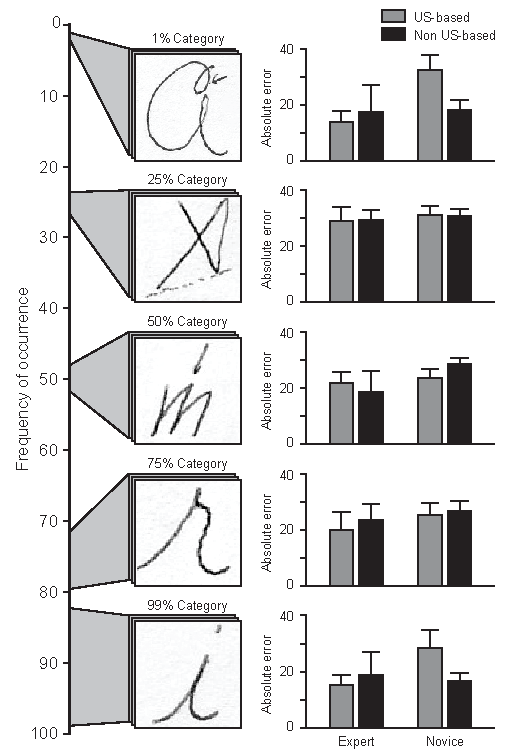
\includegraphics[scale=1]{handwritingexpertise.pdf}
\caption{Stimuli and results. On each trial, participants were presented an image and verbal description of a handwriting feature exemplar. They were asked to estimate the percentage of the US population of adult writers who had the feature in their handwriting. The handwriting features varied according to case (upper or lower), style (cursive or printed) and occurrence categories (1\% - top row, 25\%, 50\%, 75\% and 99\% - bottom row). The range of occurrence probabilities in each category is indicated on the left figure axis. The graphs on the right show experts' and novices' mean absolute error for each occurrence category by country (US or non-US). Error bars represent 95\% within-cell confidence intervals.}
\label{prettypic}
\end{center}
\end{figure}


% ----------------------------------
\section{Method}

\subsection{Participants}

One-hundred and fifty participants were recruited from forensic laboratories, mailing lists and universities via email invitation. Participants not completing the experiment or not providing complete professional practice information in order for their expertise to be determined were excluded ($n = 52$). Two handwriting specialists who had not produced any expert reports or statements and one who was involved in the NIJ project were also excluded. The final sample comprised eighteen court-practicing handwriting specialists (henceforth `experts'; $M = 149.9$ investigative and court reports from 2010-2014, Range = 9--1285; 8 US-based, 10 not) and 77 participants reporting no training, study or experience in handwriting analysis (36 US-based, 41 not). The participants that were not US-based were located in Australia (46.3\%), Canada (3.2\%), the Netherlands (2.1\%), South Africa (1.1\%) or Germany (1.1\%). A \$100 iTunes voucher was offered for the most accurate performance. Materials and data are available at \verb#https://osf.io/n2g4v/#.

% insert the screenshot
\begin{figure}[p]
\begin{center}
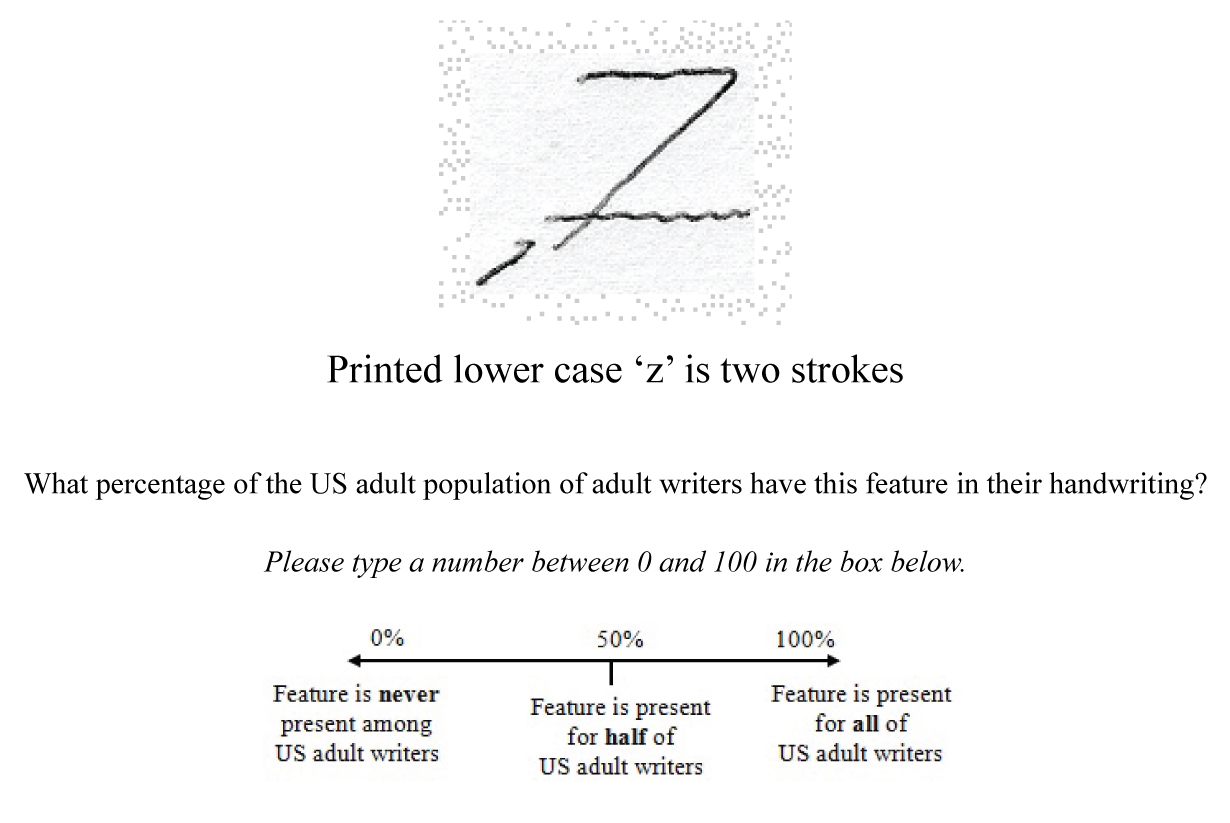
\includegraphics[scale=.3]{taskfigure2.jpg}
\caption{Screenshot illustrating the task presented to participants.}
\label{screenshot}
\end{center}
\end{figure}

% insert the histogram
\begin{figure}[p]
\begin{center}
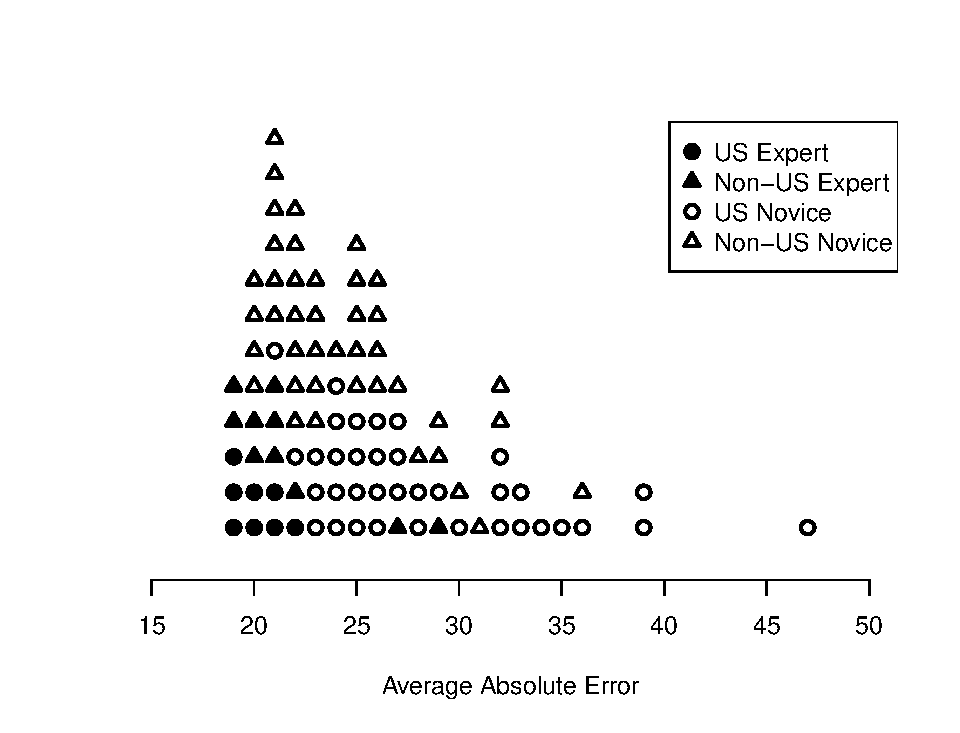
\includegraphics[scale=.7]{performance.pdf}
\caption{Histogram showing the overall accuracy of every participant, defined as the average absolute error across the 60 features. Each marker represents a single participant, with the color indicating expertise level (black = expert, white = novice) and shape indicating country (circle = US, triangle = non-US).}
\label{performance}
\end{center}
\end{figure}

\subsection{Stimuli}

Participants were presented exemplars of handwriting features selected from the NIJ database \cite{johnson2016measuring}. Sixty feature exemplars (30 cursive and 30 printed handwritten forms) were selected, 12 with probabilities closest to each of five frequencies of occurrence: 1\%, 25\%, 50\%, 75\% and 99\%. The range of probabilities within each category was determined by the available exemplars.

\subsection{Procedure}

Recruitment was necessarily time-limited and completed during the two weeks prior to the public release of the NIJ estimates. The task itself was straightforward: on every trial participants were presented a feature and asked  ``what percentage of the US population of adult writers have this feature in their handwriting?'' using a number from 0 (never present) to 100 (present for all). On each trial, participants were shown images of handwritten letters and directed to the feature by text descriptions below (see Figure~\ref{screenshot}). After completing all 60 trials, participants provided demographic and professional information.



% ----------------------------------
\section{Results}

The midpoint of the NIJ estimate range was subtracted from participant estimates to calculate absolute error for each trial. The results, averaged within-participant, are shown in Figure~\ref{performance}. To illustrate how these results depend on the handwriting feature itself, Figure~\ref{prettypic} depicts the average error for the experts and novices, broken down by country of origin (US and non-US) and by rarity of feature (averaged within category).

\subsection{Overall accuracy}

From an applied perspective, the critical question to ask is whether the expert judges are more {\it accurate} than novices, and our initial (planned) analyses consider this issue first. To that end we adopted a Bayesian linear mixed model approach, using the BayesFactor package in R \cite{morey2015}, with the absolute magnitude of the error on every trial used as the dependent variable, and incorporating a random effect term to capture variability across the 95 participants and another to capture variability across the 60 features.

When analyzed in this fashion there is strong evidence (Bayes factor 39:1 against the baseline model including only the random effects) that the expert judges were more accurate -- average error 21\% on any given trial -- than the novices, who produced errors of 26\% on average. However, the best performing model was the `full' model that considered all four groups (US experts, US novices, non-US experts, non-US novices) separately, with a Bayes factor of 300:1 against the baseline and 3.7:1 against a model that includes both main effects and no interaction. Consistent with this, the data show a clear ordering: the most accurate group were the US experts (20\% error), followed by the non-US experts (22\% error). The novices were both somewhat worse, but curiously the non-US novices performed better (24\% error) than the US novices (28\% error).

% insert the examples figure
\begin{figure}[p]
\begin{center}
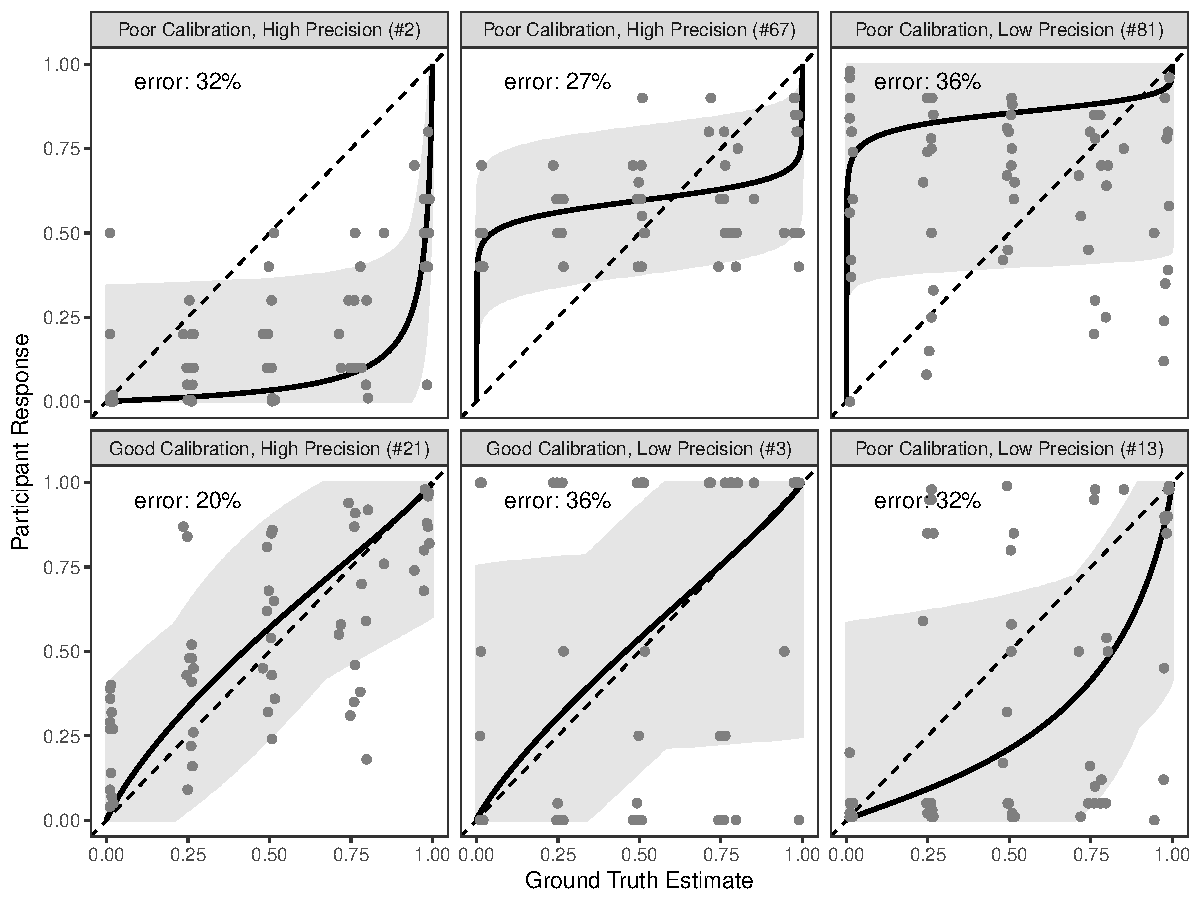
\includegraphics[scale=.7]{examples.pdf} \vspace*{6pt}
\caption{Illustration of how responses vary across individuals. Each panel represents data from a single person, with their overall error rate listed in the top left. Dots depict the response given by each person (y-axis) as a function of the ground truth probability for each item (x-axis). Solid lines depict the estimated calibration function that relates true probability to subjective probability for each person (dashed lines show perfect calibration), and the shaded areas depict 75\% prediction intervals for each person. Some participants display good calibration (\#21, \#3), illustrated by the fact that the solid line lies close to the dashed line, while others do not (\#2, \#67, \#13, \#81). Some participants are relatively precise (\#2, \#21, \#67) and have narrower prediction intervals than their less precise counterparts (\#3, \#13, \#81). Finally, miscalibration can take different forms, with some participants responding in a way that is consistently too high (\#2, \#13) or too low (\#81), and others responding in the middle for almost all items (\#67).}
\label{examples}
\end{center}
\end{figure}

\begin{figure}[t]
\begin{center}
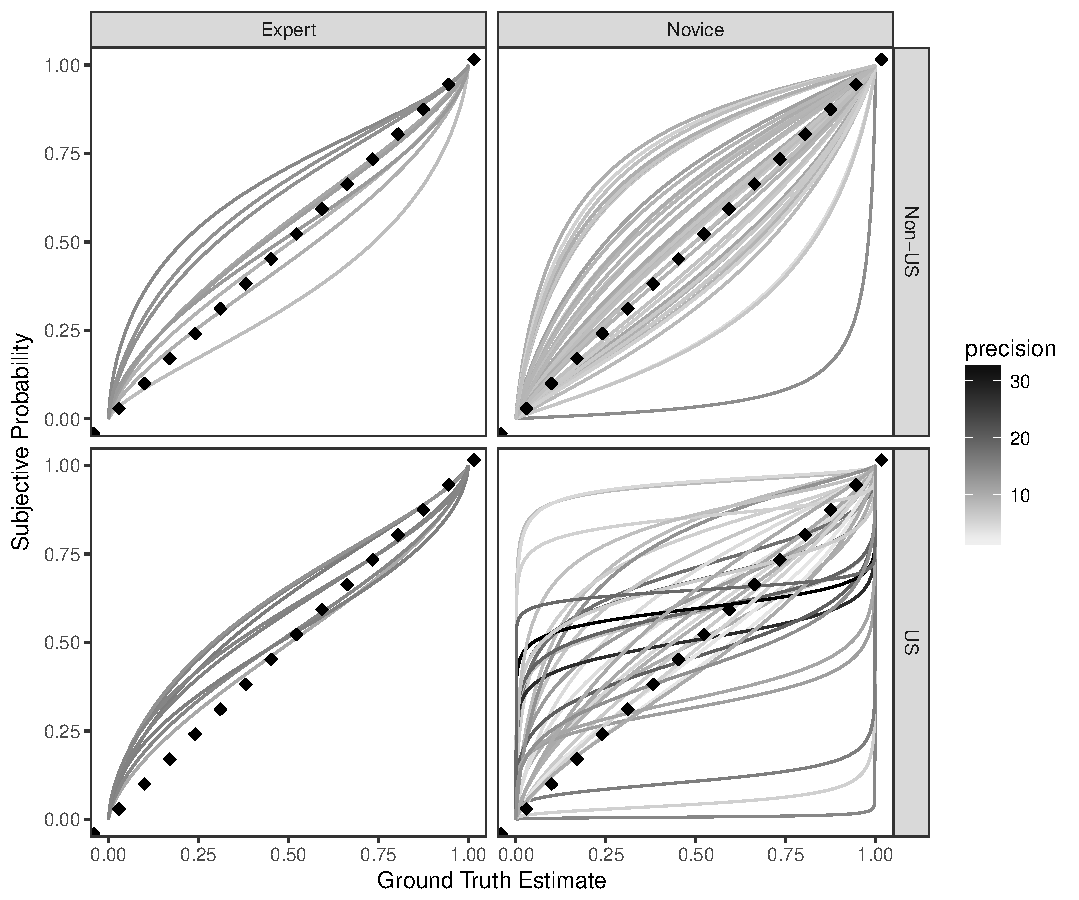
\includegraphics[scale=.7]{calibrationcurves.pdf}
\vspace*{6pt}
\caption{Estimated calibration curves for all 94 participants, plotted separately by expertise status and geographical location. The shading of each curve represents the estimated precision, with darker curves corresponding to more precise responders.}
\label{calibrationcurves}
\end{center}
\end{figure}


% ----------------------------------
\subsection{Estimating individual expert knowledge}

While it is reassuring that handwriting experts perform better on the judgment task than novices, the specific pattern of results -- in which an interaction between expertise and country is observed -- requires some deeper explanation. How does it transpire that experts from the US outperformed experts from outside the US, whereas US novices appeared to perform worse than non-US novices? Do forensic handwriting examiners possess superior knowledge of the underlying probabilities, are they more precise in how they report their knowledge, or both?

To investigate these questions, we adopt a hierarchical Bayesian approach \cite<e.g.>{merkle2010calibrating,lee2014using} that seeks to distinguish between different kinds of errors in individual responses. As is often noted in statistics \cite<e.g.,>{pearson1902mathematical,cochran1968errors} the error associated with any measurement can be decomposed into different sources. For instance, researchers interested in probability judgment often estimate a ``calibration curve'' \cite<e.g.>{Budescu2011} that captures the tendency for judgments to reflect systematic bias, as opposed to the idiosyncratic variance associated with imprecise judgments. Inspired by recent work on expert aggregation models \cite<e.g.>{merkle2010calibrating,lee2014using}, we explore these questions with the help of a hierarchical Bayesian analysis. If $x_k$ denotes the true probability of handwriting feature $k$, we adopt a two-parameter version of the calibration function used by \citeA{lee2014using},
\begin{eqnarray*}
\psi_{ik} &=& \delta_i \log \frac{x_k}{1-x_k} + \log\frac{c_i}{1-c_i}\\
\mu_{ik} &=& \frac{\exp(\psi_{ik})}{1+\exp(\psi_{ik})}
\end{eqnarray*}
In this expression, $\mu_{ik}$ denotes the subjective probability that person $i$ assigns to feature $k$, and it depends on two  parameters: the calibration $\delta_i$ describes the extent to which all subjective probabilities for the $i$-th person are biased towards some criterion value, specified by the parameter $c_i$. This calibration curve describes the \textit{systematic} error associated with the $i$-th participant. However, to capture the idea that responses $y_{ik}$ also reflect unsystematic noise, we assume that these responses are drawn from normal distribution with mean $\mu_{ik}$,  a standard deviation $\sigma_i$ that is inversely related to the \textit{precision} $1/\sqrt{\tau_{i}}$ of the $i$-th participant, truncated to lie on the range [0,1]:
$$
y_{ik} \sim \mbox{TruncNorm}(\mu_{ik},\sigma_{i}^2,0,1)
$$
For any given participant, the key quantities are therefore the parameters that describe their calibration function ($\delta_i$, $c_i$) and the precision parameter $\tau_i$ that characterizes the amount of noise in their responses. The model was implemented in JAGS \cite{plummer2003jags} and incorporated hierarchical priors over $\delta$, $c$ and $\tau$: see Appendix for detail.

% The hierarchical Bayesian calibration model used in the main text is specified as follows. Let $x_k \in [0,1]$  denote the true frequency of the $k$-th feature, and let $y_{ik} \in [0,1]$ denote the judged frequency of  feature $k$ produced by $i$-th participant. The main text describes a two-parameter calibration function,
% \begin{eqnarray*}
% \psi_{ik} &=& \delta_i \log \frac{x_k}{1-x_k} + \log\frac{c_i}{1-c_i}\\
% \mu_{ik} &=& \frac{\exp(\psi_{ik})}{1+\exp(\psi_{ik})}
% \end{eqnarray*}
% and we assume that the response is sampled from a truncated normal distribution
% $$
% y_{ik} \sim \mbox{TruncNorm}(\mu_{ik},\sigma_{i}^2,0,1)
% $$
% where the standard deviation $\sigma_{ik}$ is related to the precision via $\tau_{ik} = 1/\sigma_{ik}^2$, and notation above indicates that the distribution is truncated below at 0 and above at 1.


The critical characteristic of this model is that it allows us to distinguish {\it systematic miscalibration} from {\it imprecise responding}. To illustrate the importance of this distinction empirically, Figure~\ref{examples} displays the raw responses, average absolute error, estimated calibration curves and degree of response precision for six participants. As is clear from inspection, both sources of error matter: participants \#3 and \#21 are both extremely well calibrated, but they differ considerably in their precision. Participant \#3 does not make fine-grained distinctions in their responding, and as a consequence they sometimes make very large errors (e.g., rating a feature that has probability .01 as having probability 1), whereas the responses from participant \#21 tend to cluster much more tightly around the true value. Similarly, while the responses of participants \#2 and \#67 are almost as precise as those given by participant \#21, neither one is particularly well calibrated and their responses are not strongly related to the true probabilities.

Moreover, these plots highlight the manner in which the overall error rate is not always the best guide as to expertise. On the one hand, participant \#21 has the lowest error rate due to the fact that they have good calibration and high precision; and conversely, participant \#81 has very high error due to their poor calibration and low precision. On the other hand, the imprecise responding of participant \#3 leads to a very high error rate despite being very well calibrated. Arguably the responses of participant \#3 reflect the ground truth better than participant \#67 -- who always provides responses in the middle of the range -- even though the latter has a much lower error.

To illustrate this point more generally, Figure~\ref{calibrationcurves} plots the estimated calibration curve for all 94 participants, grouped by expertise and geographical location, with the shading of each curve representing the estimated precision of that participant.\footnote{In this figure, the values on x-axis are the ground truth values taken from \protect\citeA{johnson2016measuring}. Later in the paper we introduce a version of the model that treats the feature probabilities as unknown parameters: the calibration curves produced by that model are qualitatively the same as the curves plotted here.} Overall, it is clear that the expert respondents are better calibrated than novices, with the curves on the left of the figure tending to sit closer to the dotted line than those on the right. Formally, we assign each person a calibration score corresponding to the sum squared deviation (across all 60 items) between the estimated subjective probability $\mu_{ik}$ and the true value $x_k$, and construct 95\% credible intervals for the average difference in calibration scores between the members of different groups.\footnote{As a subtle point, note that these intervals are constructed by treating the set of participants in each group as a fixed effect rather than a random effect, and as such we report the credible interval for the mean calibration difference for these {\it specific} participants, rather than attempting to draw inferences about a larger hypothetical population. This is a deliberate choice insofar as we are uncertain what larger population one ought to generalize to in this instance -- it should be noted however that the credible intervals reported here necessarily correspond to a modest claim about these specific people rather than a more general claim about experts and novices.} The expert respondents were indeed better calibrated than novices, for both the US based participants (CI$_{95}$ = [-5.4,-3.8]) and non-US participants (CI$_{95}$ = [-1.5, -.007], though for the non-US participants the effect is modest. Similarly, we observe an difference in precision between experts and novices. Using a similar precision score that computes the sum squared deviation between the estimated subjective probability $\mu_{ik}$ and the response $y_{ik}$ we find between experts and novices for both the US based (CI$_{95}$ = [-2.3, -1.2]) and non-US based respondents (CI$_{95}$ = [-2.0, -1.0]).\footnote{The differences between the US experts and non-US experts are more difficult to characterize: different modeling assumptions produced slightly different answers for this question, beyond the original finding that US experts performed somewhat better overall.}

\subsection{Extracting wisdom from the forensic crowd}

A natural question to ask of our data is whether there is a ``wisdom of the crowd'' effect \cite{surowiecki2005wisdom}, in which it might be possible to aggregate the predictions of multiple participants to produce better judgments on the whole. Our sample includes a small number of real world experts and a much larger number of novices, and as Figure~\ref{calibrationcurves} illustrates, they differ dramatically in calibration and precision. Is it possible to aggregate the responses of these participants in a way that produces more accurate predictions than any individual expert? Does the inclusion of many poorly calibrated and imprecise novices hurt the performance of an expert aggregation model? We turn now to these questions.

Figure~\ref{modelperformance} plots the performance of two different methods of aggregating participant responses, applied to three different versions of the data: one where we included all 94 participants, one where we used responses from the 17 experts, and a third where we used only the 8 US-based experts. Using the averaging method (near right), the crowd prediction is the average of each individual prediction. As the figure illustrates, this method does not yield a wisdom of crowds effect when the novices are included in the data. Using the average response of all 94 participants yields an average prediction error of 18.6\%, slightly worse than the best individual participant in Figure~\ref{performance} whose error was 18.5\%. Once the novices are removed, the prediction error falls to 16.8\% (all experts) or 16.6\% (US experts only). As the left panels of Figure~\ref{modelperformance} illustrate, a decrease of 2\% is about the same size as the difference between the best expert (18.5\% error) and the median expert (20.4\%).

One potentially problematic issue with the averaging approach is that it only works when the very poorly performing novices are removed from the data set - in many real world situations it is not known a priori who is truly expert and who is not. We consider two methods for addressing this: the first is to rely on a robust estimator of central tendency such as the median, instead of using the arithmetic mean. As shown in Figure~\ref{modelperformance}, aggregation via the median produces better performance regardless of whether US experts (16.4\%), all experts (16.1\%) or all participants (15.7\%) are included. The second method is to adopt a hierarchical Bayesian approach based on \citeA{lee2014using}, using the more general calibration functions discussed in the previous section. The advantage of this approach is that it automatically estimates the response precision for each person, and learns in an unsupervised way which participants to weight most highly. As illustrated in the far right of Figure~\ref{modelperformance}, this model makes better predictions than the averaging method or the median response method: using only the US experts the prediction error is 15.1\%, which falls slightly to 14.9\% when all experts are used, and improves slightly further to 14.7\% when the novices are included. In other words, not only is the hierarchical Bayes method robust to the presence of novices, it is able to use their predictions to perform better than it does if only the experts are considered and yields better estimates than simple robust methods such as median response.

Finally, to understand why the Bayesian aggregation model performs better than the simpler averaging method, Figure~\ref{aggregation} plots the model based estimates against the average human response (left) and compares both of these prediction methods to the ground truth estimated from the NIJ data (middle and right panels). As shown in the left panel, the main thing that the model has learned is to transform the average estimates via a non-linear calibration function that closely resembles curves used in standard theoretical models \cite{prelec1998probability}, though as illustrated in Figure~\ref{examples} individual subject calibration curves often depart quite substantially from this shape. This has differential effects depending on the true frequency of the handwriting feature in question: for very rare and very common features, the model reverses the regression to the mean effect, and so the Bayesian model produces much better estimates for these items \cite<see also>{satopaa2014combining}. The overall result is that the model estimates produce a much better prediction about the ground truth (middle panel) than the averaging method (right panel).



% model performance
\begin{figure}[p]
\begin{center}
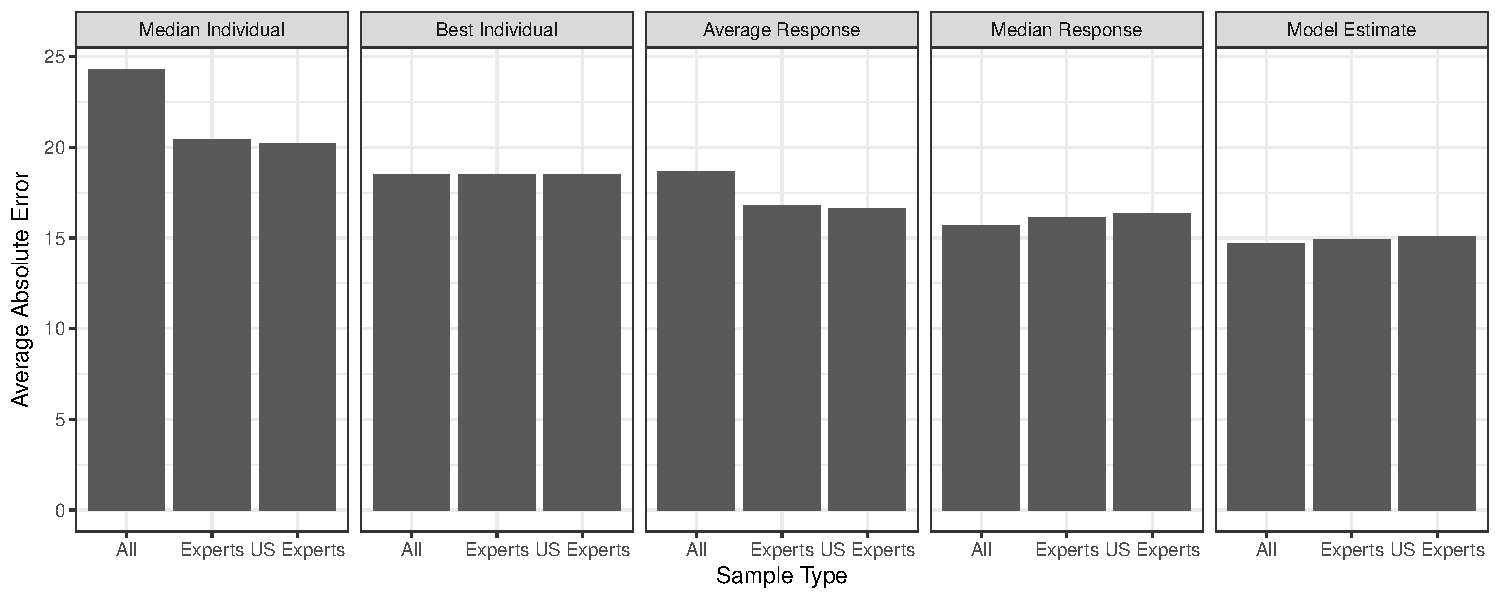
\includegraphics[scale=.6]{modelperformance.pdf}
\caption{Performance of the aggregation model (far right), when compared to simpler aggregation approaches that averages responses (middle) or takes the median response (near right). For comparison purposes, both are plotted against the performance of the best individual participant (near left), and the median performance of all respondents (far left). Within each panel, three versions are plotted: one where we included all 94 participants, one where we used responses from the 17 experts, and a third where we used only the 8 US-based experts.}
\label{modelperformance}
\end{center}
\end{figure}


% aggregation
\begin{figure}[p]
\begin{center}
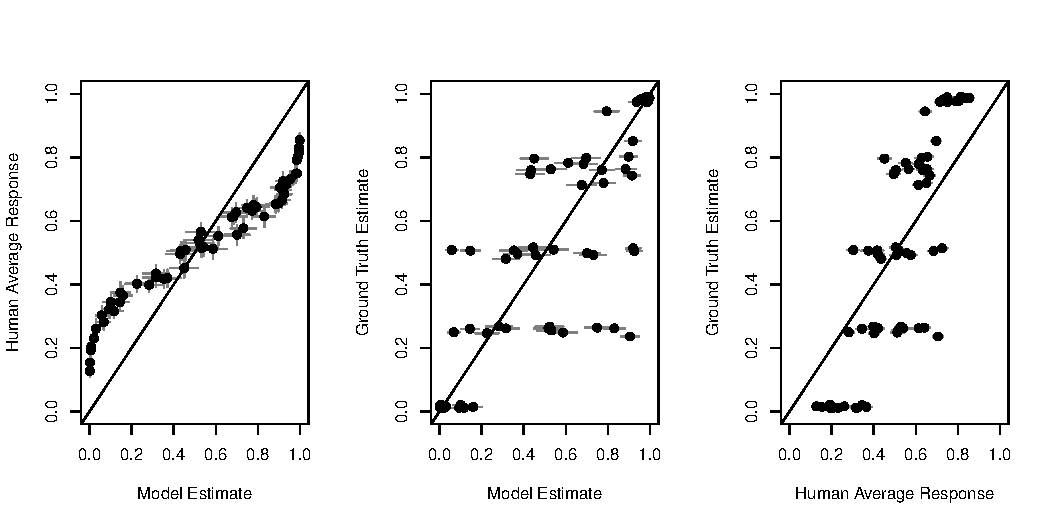
\includegraphics[scale=.9]{aggregation.pdf}
\caption{Aggregating expert predictions. Pairwise comparisons between the ground truth estimated from the NIJ data, the average response of human participants, and the estimates extracted via the hierarchical Bayesian model.}
\label{aggregation}
\end{center}
\end{figure}



% ----------------------------------
\section{Conclusions}

The assessment of expert performance is a problem of considerable  importance. Besides the obvious theoretical questions pertaining to the nature of expertise \cite<e.g.>{weiss2003empirical,ericsson1996expert}, a variety of legal, professional and industrial fields are substantially reliant on human expert judgment. For the specific domain of forensic handwriting examination the legal implications are the most pressing. In this respect our findings are mixed.

On the one hand, there is some evidence that handwriting experts will be able to estimate the frequency of occurrence for handwriting features better than novices. However, even the single best performing participant produced an average deviation of 18.5\% from the true value. On the other hand, this number is considerably lower than would be expected by chance (25\%) if people possessed no relevant knowledge and simply responded with .5 on every trial, and using modern Bayesian methods to aggregate the predictions of the experts this can be reduced further to 14.7\% error.

In short, these results provide some of the first evidence of naturalistic visual statistical learning in the context of forensic feature comparison. However, we suggest that a cautious approach should be taken before endorsing the use of experience-based likelihood ratios for forensic purposes in the future.

% ----------------------------------

% insert reference list
\bibliography{references}
\bibliographystyle{apacite}

\section{Appendix}

\noindent
The hierarchical Bayesian calibration model used in the main text is specified as follows. Let $x_k \in [0,1]$  denote the true frequency of the $k$-th feature, and let $y_{ik} \in [0,1]$ denote the judged frequency of  feature $k$ produced by $i$-th participant. The main text describes a two-parameter calibration function,
\begin{eqnarray*}
\psi_{ik} &=& \delta_i \log \frac{x_k}{1-x_k} + \log\frac{c_i}{1-c_i}\\
\mu_{ik} &=& \frac{\exp(\psi_{ik})}{1+\exp(\psi_{ik})}
\end{eqnarray*}
and we assume that the response is sampled from a truncated normal distribution
$$
y_{ik} \sim \mbox{TruncNorm}(\mu_{ik},\sigma_{i}^2,0,1)
$$
where the standard deviation $\sigma_{ik}$ is related to the precision via $\tau_{ik} = 1/\sigma_{ik}^2$, and notation above indicates that the distribution is truncated below at 0 and above at 1.

To accommodate individual and group differences we assume that the precision $\tau_{i}$, calibration $\delta_i$ and criterion $c_i$ parameters are sampled from a population distribution that may have slightly parameters as a function of the group $g_i$ (e.g., US expert) to which the expert belongs. For each group $g$ the calibration parameter $\delta$ is sampled from a Gaussian distribution with unknown mean $\mu_{\delta,g}$ and precision $\tau_{\delta,g}$, truncated to lie between 0 and 1. A similar approach is applied to the precision and criterion parameters, yielding the following model at the group level:
\begin{eqnarray*}
\delta_i | g_i=g & \sim & \mbox{TruncNorm}(\mu_{\delta,g}, 1/\tau_{\delta,g},0,1) \\
c_i | g_i=g & \sim & \mbox{TruncNorm}(\mu_{c,g}, 1/\tau_{c,g},0,1) \\
\tau_i | g_i=g & \sim & \mbox{TruncNorm}(\mu_{\tau,g}, 1/\tau_{\tau,g},0,\infty)
\end{eqnarray*}
To capture the intuition that the various groups may be somewhat similar to one another, the group level parameters are assumed to be drawn from a higher level population distribution, again assumed to be a truncated normal distribution
\begin{eqnarray*}
\mu_{\delta,g} & \sim &  \mbox{TruncNorm}(\mu^\prime_1,1/\tau^\prime_1,0,1) \\
\mu_{c,g} & \sim & \mbox{TruncNorm}(\mu^\prime_2,1/\tau^\prime_2,0,1) \\
\mu_{\tau,g} & \sim & \mbox{TruncNorm}(\mu^\prime_3,1/\tau^\prime_3,0,\infty) \\
\tau_{\delta,g} & \sim & \mbox{TruncNorm}(\mu^\prime_4,1/\tau^\prime_4,0,\infty) \\
\tau_{c,g} & \sim & \mbox{TruncNorm}(\mu^\prime_5,1/\tau^\prime_5,0,\infty) \\
\tau_{\tau,g} & \sim & \mbox{TruncNorm}(\mu^\prime_6,1/\tau^\prime_6,0,\infty)
\end{eqnarray*}
Finally, non-informative hyperpriors were adopted to describe the prior over the population level parameters $\mu^\prime$ and $\tau^\prime$: Gamma(.01,.01) distributions for parameters lower bounded at zero, and uniform priors for parameters that lie between 0 and 1.
\end{document}




